\chapter{Contexto}
\label{chap:contexto}

\lettrine{N}{este} apartado introdúcense o contexto relevante a este traballo que provee os conceptos básicos necesarios para a súa comprensión.
Para elo descríbese o campo da oftalmoloxía e a imaxe médica, así como o estado da arte en aliñamento de imaxes.
\section{Oftalmoloxía}
\label{sec:Oftalmoloxía}
A oftalmoloxía é a especialidade médica que se encarga do estudo e tratamento do ollo e os seus trastornos.
 O ollo humano é un dos órganos dos que mais dependemos e maior cantidade de información sensorial aporta, e en consecuencia tamén é un dos mais complexos do noso corpo.
 Así mesmo, é unha das rexións que máis datos aporta sobre o estado de saúde do paciente, xa que permite observar directamente os vasos sanguíneos e o tecido neuronal "in-vivo".
 Isto permite a detección temprana de enfermidades, que poden ser diagnosticadas mediante a observación da retina.
\subsection{Anatomía do ollo humano}
\label{subsec:Anatomía do ollo humano}
O ollo encargase de captar a luz e transformala en impulsos eléctricos que se envían ao cerebro.
 Esta información é interpretada polo cerebro, que mediante mecanismos como a atención e a memoria, permite a percepción visual.
 \dots

\subsection{Imaxe oftalmolóxica}
\label{subsec:Imaxe oftalmolóxica}
Existen diversas modalidades de imaxe médica que permiten observar o ollo, cada unha con diferentes propiedades e aplicacións. 
As mais utilizadas son a fotografía de fondo de ollo (retinografía), a tomografía de coherencia óptica (OCT) e a angiografía con fluoresceína.

\subsection{Retinografía}
\label{subsec:Retinografía}
Este traballo céntrase na retinografía xa que é a mais común.
Isto é débese en gran parte á súa accesibilidade, requerindo equipo maís barato e menor entrenamento comparada cas outras modalidades
Ademais, é unha técnica non invasiva e rápida de realizar, o que a fai preferible na maioría dos casos.

Para realizala utilízase unha cámara especial denominada retinógrafo, e xeralmente require da previa dilatación da pupila do paciente.
Desta forma permítese maior entrada de luz nos ollos, o que provoca unha mellor visualización da retina e mellora a calidade da imaxe.
Un especialista pode analizar a retinografía para detectar signos de enfermidades como a retinopatía diabética, a hipertensión ou a degeneración macular.

imagenFIRE

\section{Rexistro de imaxes}
\label{sec:Rexistro de imaxes}
O rexistro de imaxes é un proceso que consiste en, sobre dúas ou mais imaxes, determinar a correspondencia espacial entre elas e alinealas nun sistema de coordenadas común.
Así conséguese que as características de interese se atopen na mesma posición.
Este proceso pode empregarse para comparar imaxes dun mesmo paciente tomadas en distintos momentos, en distintas modelidades ou para comparar entre diferentes pacientes.
Isto permite a revisión do avance dunha enfermidade ao longo do tempo, a fusión de imaxes de distintas modalidades ou a detección de patróns comúns en distintos individuos.

No caso de trabllar con dúas imaxes, a imaxe de referencia denomínase imaxe fixa (f) e a imaxe que se quere rexistrar imaxe móbil(m).
Ata recentemente, gran parte do traballo de rexistro facíase de forma manual por expertos, 
e dependía das habilidades do profesional para detectar as características de interese e realizar o aliñamento.
Isto facía que o proceso fose lento e propenso a erros, ademais de pouco práctico para grandes volumes de imaxes.

Dependendo do tipo de transformación esta pode ser clasificada en ríxida, afín ou deformable.
A ríxida tan só permite rotación e traslación, mentres que a afín permite ademais escalado e cizallamento.
Ámbas transformacións poden ser representadas por unha matriz de 2 dimensións xa que son deformacións lineais.
Ao contrario, a transformación deformable é non lineal, polo que require dunha dimensión adicional ás da imaxe a rexistrar (unha imaxe de 2d require unha matriz 3d).
Esta matriz denomínase campo de vectores de deformación (DFV), e permite representar deformacións locais na imaxe, facendoa moito mais flexible para representar transformacións complexas.

\subsection{Métodos de aliñamento de imaxes automáticos}
\label{subsec:Métodos de aliñamento de imaxes automáticos}
Existen diversos métodos para realizar aliñamento de imaxes, que poden estar automatizados en maior ou menor medida.


\dots

\subsection{Estado da arte}
\label{subsec:Estado da arte}


Tradicionalmente impregáronse métodos iterativos baseádos na extracción de características 
seguido dun proceso de optimización entre cada par de imaxes. 
Isto require recoñecer as características de interese en cada imaxe e utilizar unha métrica de similitude 
para determinar a calidade do rexistro.
O proceso consiste en calcular o grado de semellanza entre as imaxes e 
actualizar os parámetros da transformación de forma iterativa ata que se cumpran os criterios de terminación.
O resultado final pode ser os parámetros da transformación ou a imaxe fusionada.

\begin{figure}[hp!]
    \centering
    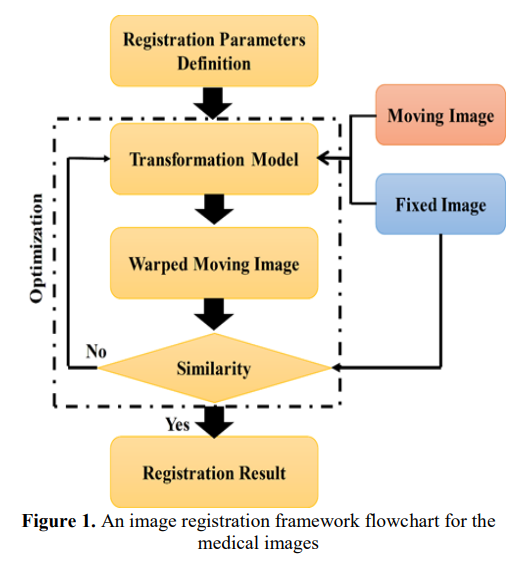
\includegraphics[width=0.75\textwidth]{imaxes/iterativoSubrato.png}
    \caption{Pé de imaxe descritivo}
    \label{fig:exemplo}
  \end{figure}
  

\dots
A principal desventaxa destes métodos é a súa lentitude.

\subsection{Métodos de aprendizaxe profunda}
\label{subsec:Métodos de aprendizaxe profunda}

Ca chegada dos métodos de aprendizaxe profunda á imaxe médica, comezaron a empregarse redes neuronais para realizar o aliñamento de imaxes.
Estos métodos tenden a ser mais rápidos que os métodos convencionais, a custo de algo de precisión. 
Ademais, estos métodos requiren dunha gran cantidade de datos para ser adestrados, 
o que pode ser unha desventaxa xa que en moitos casos non se dispoñen de bases de datos anotadas do tamaño necesario.

Unha aproximación común é empregar estes conxuntos de datos para optimizar unha CNN que,
 dadas dúas imaxes novas e non vistas, predice o DFV correspondente.

Durante o proceso de entrenamento, a rede ten acceso aos DFVs ca deformación correcta,
 ou pódense obter indirectamente a través da optimización dunha métrica de similitude de imaxes [].

Existen moitas extensións a esta aproximación, como o uso de múltiples etapas ou o uso de redes adversarias durante o entrenamento.

Tamén se propuxeron métodos híbridos que combinan a optimización iterativa ca aprendizaxe profunda, 
entrenando unha CNN nova por cada parella de imaxes. Desta forma conséguese evitar a necesidade de grandes conxuntos de datos para o adestramento.

Os métodos de aprendizaxe profunda poden ser clasificados en dous tipos según se requiran de DFVs anotados ou non na etapa de entrenamento: 
supervisados (requíren de DFVs anotados) e non supervisados (non requíren de DFVs anotados).

\subsubsection{Métodos Supervisados}
\label{subsubsec:Métodos Supervisados}

Existen dúas subcategorías según o grado de supervisión utilizado na etapa de entrenamento: totalmente supervisados ou débilmente supervisados.
O rexistro totalmente supervisado fai uso de DVFs de referencia para supervisar o proceso de aprendizaxe.
 O termo de perda adoita basearse na discrepancia entre os DVFs de referencia e os DVFs predicidos.
 En lugar de empregar DVFs de referencia, o rexistro débilmente supervisado pode utilizar outras etiquetas de referencia implícitas.
 Estas etiquetas non se basan en datos explícitos como os DFVs, senón que utilizan información indirecta para guiar o proceso de rexistro, como a semellanza entre as imaxes ou restricións baseadas na forma ou límites anatómicos das estruturas.
 Máis de dous tipos de datos de referencia son frecuentemente utilizados para adestrar modelos de rexistro débilmente supervisados.
\dots

\subsubsection{Métodos Non Supervisados}
\label{subsubsec:Métodos Non Supervisados}

A creación de conxuntos de DFVs anotados é un proceso laborioso e costoso, polo que os métodos de rexistro non supervisados son de gran interese.
Xa que a imaxen fixa e a imaxe móbil xa conteñen a información necesaria para un rexistro correcto, os métodos non supervisados parecen mais adecuados para a tarefa de rexistro.
De forma similar aos métodos iterativos, é común empregar unha métrica de similitude entre as imaxes xunto con un termo de regularización para guiar o proceso de optimización evitando caer en transformación non realistas.
O rexistro non supervisado de imaxes médicas utilizando GANs é unha subcategoría desta técnica.

\subsubsection{Métodos baseasdos en Reinforcement Learning}
\label{subsubsec:Métodos baseados en Reinforcement Learning}



\cite{wolterink2021implicit} propuxeron un método de aliñamento de imaxes baseado en redes de representación implícita,
 que é no que se basa este traballo e descríbese en maior detalle na seguinte sección \ref{subsec:IDIR}.

\subsection{IDIR}
\label{subsec:IDIR}
IDIR (Implicit Deformable Image Registration) é un método de aliñamento de imaxes baseado en redes neuronais. 
A súa principal diferenza frente a unha rede convolucional tradicional é que, 
en lugar de predicir a transformación entre imaxes, optimízase unha rede para esta mesma represente esta transformación.


\subsubsection{Representación Neuronais Implícitas}
\label{subsubsec:Representación Neuronais Implícitas}

É común empregar redes convolucionais para o aliñamento de imaxes,
 tipicamente como un operador que mapea entre unha parella de imaxes e o DFV.

O que \cite{wolterink2021implicit} propón é optimizar directamente o DFV facenda uso
 dunha representación implícita, de forma que a deformación está representada nos propios pesos dunha MLP.

Según o teorema de aproximación universal (Hornik et al., 1989), calquera función ben comportada
 pode ser descrita con precisión arbitrariamente alta por unha rede neuronal apropiada. 
 Na nosa aplicación, a rede pode variar en profundidade ou ancho, pero sempre terá n entradas e n saídas para transformacións en espazo euclidiano n-dimensional.




No caso do aliñamento de imaxes, buscase optimizar a función que mapea cada localización x nunha imaxe a unha localización na outra.


 \subsubsection{Método}
 \label{subsubsec:Método}

Sendo o obxetivo encontrar unha transformación espacial óptima entre a imaxe fixa e a imaxe móbil,
 é necesario obter a función de deformación  Φ(x) = u(x) + x que mapea cada coordenada x na imaxe fixa a unha coordenada na imaxe móbil, 
 de forma que a coordenada x na imaxe fixa corresponda anatomicamente á coordenada Φ(x) na imaxe móbil.
Este problema pode ser formulado como un problema de optimización onde Ldata é unha métrica de similitude entre as imaxes fixa e móbil, Lreg é un termo de regularización na transformación Φ, e α é un termo de ponderación.
\begin{equation}
    \hat{\Phi} = \operatorname*{Arg\,min}_{\Phi} L_{data}(M \circ \Phi, F) + \alpha L_{reg}(\Phi)
\end{equation}

A aportación clave é que a transformación Φ está implícitamente representada nunha rede neuronal.

Comparado cunha CNN tradicional, esta rede non recibe valores de intensidade de píxel como entrada,
 senón que recibe coordenadas espaciais (continuas) e devolve unha nova coordenada.
Xa que os pesos da rede definen a transformación, estos poden ser optimizados directamente 
facendo uso dunha métrica de similitude como función de perda.

Parametrizar a función de deformación como unha INR dentro dun MLP ten varias vantaxes para o rexistro de imaxes.
En primeiro lugar, a representación da transformación é continua e polo tanto independente da resolución da imaxe, 
grazas a iso o mesmo modelo poder ser empregado para imaxes de calquer tamaño, ao contrario dunha CNN tradicional 
que ten que ser adaptada para cada resolución.

Segundo, facelo desta forma permite aproveitar as capacidades de librerías como PyTorch para calcular os gradientes da transformación respecto das coordenadas.
Isto permite obter gradientes máis precisos que as aproximacións por diferencias finitas 
e permite aproveitar unha gran cantidade de literatura sobre regularización eficientes en imaxes médicas.

Terceiro, pódese modificar a función de activación empregada na rede para axustala ás necesidades particulares da tarefa de rexistro de imaxes.
Neural Tangent Kernel (NTK) es un concepto que describe cómo un modelo de red neuronal responde a cambios en sus parámetros durante el entrenamiento,
 e dependendo da función de activación empregada, o NTK varía e a rede pode ser máis ou menos sensible a certas deformacións.

 Finalmente, entrenaráse unha nova rede por cada parella de imaxes, sendo esta unha rede bastante pequena en comparación e precindindo así da necesidade de grandes conxuntos de datos para o seu adestramento.
 
\subsubsection{Arquitectura}
\label{subsubsec:Arquitectura}


\subsubsection{Función de activación}
\label{subsubsec:Función de activación}

Unha elección estándar para a función de activación é ReLU: σ(x) = max(0, x).
Sen embargo, as ReLUs teñen un sesgo cara a sinais de baixa frecuencia (Mildenhall et al., 2020; Tancik et al., 2020), 
 o que significa que o modelo pode ter dificultades para representar pequenas deformacións locais no rexistro de imaxes.
 
Existen varias formas de superar este sesgo, como preprocesar as coordenadas de entrada con funcións de activación periódicas (Mildenhall et al., 2020; Tancik et al., 2020) ou substituír a función de activación ReLU por unha función de activación periódica (Sitzmann et al., 2020).
Neste traballo escollemos a segunda opción, utilizando unha función de activación periódica para obter un modelo de tipo SIREN, σ(x) = sin(x).
Unha vantaxe engadida das funcións de activación periódicas nas redes SIREN é que poden ser diferenciadas varias veces, 
o que expande substancialmente o conxunto de termos de regularización que se poden empregar na rede, como veremos na seguinte sección.

\subsubsection{Termos de regularización}
\label{subsubsec:Termos de regularización}

Debido a que el registro de imágenes deformables es un problema mal planteado (ill-posed problem**), 
es común regularizar el DVF para evitar deformaciones poco realistas.
 Los métodos de registro basados en redes neuronales convolucionales (CNN) representan los DVF 
 como muestras en una cuadrícula de vóxeles, y por lo tanto, solo pueden aproximar gradientes espaciales
 mediante esquemas de diferencias finitas. Esto conlleva errores de discretización y pérdidas de precisión.

Facendo uso de representacións implícitas, todas as operación son diferenciables, e os gradientes poden
 ser computados de forma analítica en lugar de ter que aproximalos.
Utilizando ReLU como función de activación, a rede é diferenciable unha vez, mentres que utilizando
 unha función de activación periódica (como SIREN), a rede é diferenciable varias veces.
Desta forma, podemos calcular calquera número de termos de regularización e incluilos na optimización da rede.

Algúns exemplos de termos de regularización que se poden empregar son:
\begin{itemize}
    \item Jacobian regularizer: 
    O determinante Jacobiano da transformación (det ∇Φ) nunha localización x é un indicador de estiramento ou compresión local.
    Un determinante Jacobiano negativo indica que está a ocurrir folding e a transformación non será invertible.
    \dots

    \item Hyperelastic regularizer
    Tamén se póden engadir restricións ao DVF con este termo proposto por (Burger et al., 2013).
    Consiste en tres termos, un termo de lonxitude, un termo de área e un termo de volumen co obxetivo de controlar variacións nestes aspectos.
    O termo de lonxitude penaliza a variación da lonxitude dos vectores do DVF e está controlado pola matriz do Jacobiano da transformación.
    A matriz de cofactores e o determinante da matriz do Jacobiano da transformación controlan a área e o volume respectivamente, 
    penalizando o crecemento e a contracción por igual.
    \dots

    \item Bending energy penalty
    Pódese impoñer a suavidade do DVF empregando esta penalización proposta en (Rueckert et al., 1999).
    Require que as segundas derivadas do DVF sexan pequenas en todo o dominio, 
    polo que non pode ser utilizado nunha rede que utilice ReLU como función de activación (a segunda derivada de unha ReLU é sempre igual a 0).
    \dots
\end{itemize}